\documentclass[10pt,a4paper]{article}
\usepackage[T1]{fontenc}
\usepackage[scaled]{helvet}
\usepackage{cite}
\usepackage{url}
\usepackage{graphicx}
\usepackage{listings}
\usepackage{float}
\usepackage{amsmath}
\usepackage{listings}
\usepackage{color}
 
\definecolor{dkgreen}{rgb}{0,0.6,0}
\definecolor{gray}{rgb}{0.5,0.5,0.5}
\definecolor{mauve}{rgb}{0.58,0,0.82}
\lstset{ %
  language=Octave,                % the language of the code
  basicstyle=\footnotesize,           % the size of the fonts that are used for the code
  numbers=left,                   % where to put the line-numbers
  numberstyle=\tiny\color{gray},  % the style that is used for the line-numbers
  stepnumber=1,                   % the step between two line-numbers. If it's 1, each line 
                                  % will be numbered
  numbersep=5pt,                  % how far the line-numbers are from the code
  backgroundcolor=\color{white},      % choose the background color. You must add \usepackage{color}
  showspaces=false,               % show spaces adding particular underscores
  showstringspaces=true,         % underline spaces within strings
  showtabs=false,                 % show tabs within strings adding particular underscores
  frame=none,                   % adds a frame around the code
  rulecolor=\color{black},        % if not set, the frame-color may be changed on line-breaks within not-black text (e.g. commens (green here))
  tabsize=2,                      % sets default tabsize to 2 spaces
  breaklines=true,                % sets automatic line breaking
  breakatwhitespace=false,        % sets if automatic breaks should only happen at whitespace
  keywordstyle=\color{blue},          % keyword style
  commentstyle=\color{dkgreen},       % comment style
  stringstyle=\color{mauve},         % string literal style
  escapeinside={\%*}{*)},            % if you want to add LaTeX within your code
  morekeywords={*,...}               % if you want to add more keywords to the set
}
\usepackage{amssymb}
\usepackage{fancyhdr}
\usepackage{lastpage}
\floatstyle{boxed} 
\restylefloat{figure}
\renewcommand*\familydefault{\sfdefault}
\title{Introduction to Algorithms}
\author{David Lynch - david.lynch@raglansoftware.com }
\begin{document}
\maketitle
\begin{abstract}
We shift or focus now from core operating systems to algorithms and data structures. Essentially, we pivot from looking at software and methods that facilitate the creation and running of programs to the actual construction of the programs themselves. We start with a gentle introduction to some primitive data-structures and put a formal framework around evaluating algorithms.
\end{abstract}
\section{Elementary Data Structures}
Dynamic sets are the fundamental structures to computer science. Strictly speaking, mathematical sets are unchanging, however in computer science it is useful to picture a set as a collection of values that actually mutates in some way over time. We make the distinction by calling these types of sets {\bf dynamic}. Algorithms may require several different types of operations to be performed on sets of data. We refer to sets that support these operations as {\bf dictionaries}. Operations that must be supported for particular dictionaries vary between data-structure, each of which will have its own set of operations that together make the structure unique. Dictionaries contain {\bf objects} of primitive data each of which is identified individually due to either their position in a set relative to the lower and upper bounds, that is by {\bf implicit key}, or by means of {\bf explicit key}. The explicit key is derived from some identiifying value or set of values that are associated with the object itself. An example implicit key is the position of an object reference in an array, whereas an explicit key may be a hash-code derived from the results of a hash function across the associated object. It is beneficial to think of dictionaries as sets of {\bf key-value pairs}. The data associated with an objeect that is unused by the set implementation itself is known as {\bf satellite data}. So, consider the example of an array of bank accounts. The key is the implicit position in the array, which maps to an object reference that resolves to the account number, name and balance. 
\newline\newline
If $S$ is a possibly ordered set and $k$ is a {\bf key} that points to some object $x$, anything that modifies the contents of $S$ is a {\bf modifying operation}. Otherwise, if the set is not ordered, the operation is known as a {\bf query}. Figure \ref{operations} shows example of both types of operation.
begin{figure}
\caption{A list of common query and modifying set operations.}
\begin{center}
\begin{tabular}{| l | l | }
  Operation & Description \\
  \hline
  SEARCH($S$, $k$) & Find element with key $k$ in set $S$. \\
  INSERT($S$, $k$) & Insert key $k$ into set $S$. \\
  DELETE($S$, $k$) & Delete key $k$ from $S$. \\
  MINIMUM($S$) & Return the minimum key $k$ in $S$. \\
  MAXIMUM($S$) & Return the maximum key $k$ in $S$. \\
  SUCCESSOR($S$, k) & Return the sucessor key to $k$ in $S$. \\
  PREDECESSOR($S$, k) & Return the predecessor key to $k$ in $S$. \\
  \hline
\end{tabular}
\end{center}
\label{operations}
\end{figure}
\subsection{LIFO & FIFO Data Structures}
The simplest form of data structures we consider are {\bf stacks} and {\bf queues}. They are similar in structure, differing in how objects are placed into the set and removed from the set. A stack is a {\bf last-in, first-out} data-structure. The listing in figure \cite{stack} fleshes out operations on a stack. As is shown, the last object to get placed on the stack will be the first object to get removed from the stack at the next call to the POP remove operation. The listing in figure \cite{queue} shows conversely, the first element inserted is the first element removed from the queue given sucessive calls to the correct modifying operations. If we attempt a {\it delete} on an empty queue or stack, we will {\bf underflow} if we attempt an {\it insert} to a stack or queue that is full, we get an {\bf overflow}. As we have already seen stacks map particularly well to growth of main memory, in particular the execution trace of a program. We have already seen FIFO queues used to good effect in article 7, both in the producer consumer problem and when talking about mailboxes in article 5.
\begin{figure}
\caption{Stack operations in pseudo-code}
\begin{center}
\begin{lstlisting}
STACK-EMPTY(S)
if S.top == 0
    return TRUE
else  
    return FALSE
\end{lstlisting}
\begin{lstlisting}
STACK-FULL(S)
if S.top >= MAX_SIZE
    return TRUE
else  
    return FALSE
\end{lstlisting}
\begin{lstlisting}
PUSH(S, x)
if STACK-FULL(S)
  error "Overflow"
S.top    = S.top+1
S[S.top] = x	
\end{lstlisting}
\begin{lstlisting}
POP(S)
if STACK-EMPTY(S)
    error "Underflow"
else  
    S.top = S.top-1
return S[S.top+1]
\end{lstlisting}
\label{stack}
\end{center}
\end{figure}
\begin{figure}
\caption{Queue operations in pseudo-code}
\begin{center}
\begin{lstlisting}
ENQUEUE(Q, x)
Q[Q.tail] = x
if Q.tail == Q.length
  Q.tail = 1
else
  Q.tail = Q.tail+1
\end{lstlisting}
\begin{lstlisting}
DEQUEUE(Q)
x = Q[Q.head]
if Q.head == Q.length
  Q.head =1
else
  Q.head = Q.head+1
return x
\end{lstlisting}
\label{queue}
\end{center}
\end{figure}
\section{Linked List}
A linked list is a data structure in which objects are arranged in a linear order that is defined by properties of each {\bf node} in the list. Unlike an array, where this order is determined by proximity, a pointer to the next or previous node in the list at each element is used. In the case of a doubly linked list, pointers to both the predecessor and the sucessor nodes are kept at each node. Otherwise, if the predecessor link is omitted, the list is singly linked. Any linked list must be bound, and this can be done either by inserting $NIL$ explicitly to the predecessor of the first element and sucessor of the last element, or joining the tail and head element by means of pointers. The latter example may be a means to create a {\bf wrapped list} or more commonly {\bf ring buffer}. Linked lists may also be sorted. Figure \cite{linkedlisting} shows some operations on linked list and figure \cite{linkedgraphic} shows linked lists represented diagramatically.

\end{figure}
\begin{figure}
\caption{Operations on a Linked list}
\begin{center}
\begin{lstlisting}
LIST-SEARCH(L, k)
x = L.head
while x != NIL and x.key != k
  x = x.next
return x
\end{lstlisting}
\begin{lstlisting}
LIST-INSERT(L, x)
x.next = L.head
if L.head != NIL
  L.head.prev = x
L.head=x
x.prev=NIL
\end{lstlisting}
\begin{lstlisting}
LIST-DELETE(L, x)
if x.prev != NIL
  x.prev.next = x.next
else
  L.head = x.next
if x.next != NIL
  x.next.prev = x.prev
\end{lstlisting}
\label{linkedlisting}
\end{center}
\end{figure}
\section{Linked List}
begin{figure}
\caption{A linked and doubly linked list.\cite{OSCONCEPTS}}
\begin{center}
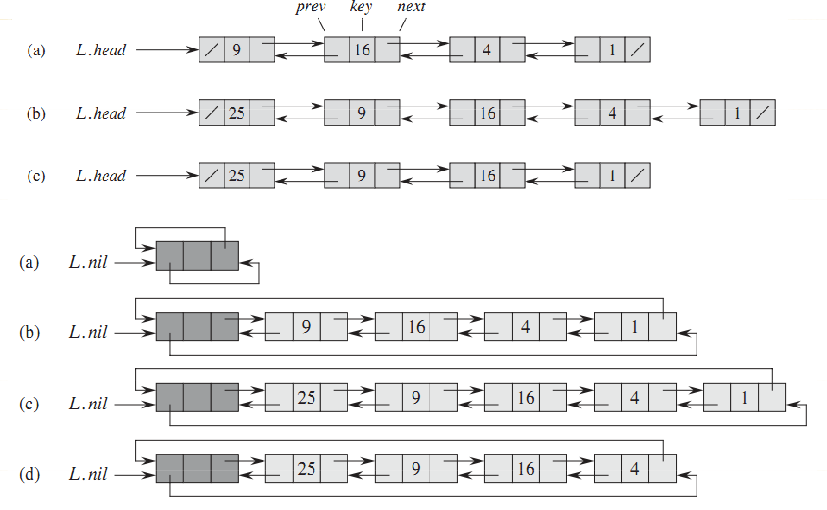
\includegraphics[scale=0.5]{../images/linkedlist.png}
\label{paging}
\end{center}
\end{figure}
\section{Trees}
We can use reference pointers and logical operations similar to that of linked lists to create rooted trees. The most elementary of these tree structures is a {\bf binary tree}. Each node of a binary tree has a possibly null ancestor and two possibly null children, left and right. This concept can be extended to create rooted trees with unbounded branching. These are known as $k-Ary$ trees, where $k$ may be fixed or totally unbounded.  


\bibliography{../biblio/techfundamentals.bib}{}
\bibliographystyle{plain}
\begin{center}
{\small \copyright  David Lynch 2012. Do not reproduce without written permission.}
\end{center}
\end{document}
